\documentclass{article}
\usepackage[utf8]{inputenc}

\title{Final Project Report: Predicting University of California Admissions Decisions}
\author{Hanna Rakhsha \and Ram Moore \and Samantha Aziz}
\date{December 1, 2019}

\usepackage{graphicx}
\usepackage{subcaption}
\usepackage{natbib}
\usepackage{indentfirst}
\graphicspath{ {./images/} }

\begin{document}

\maketitle

\section{A Note on Optical Character Recognition}
The subject of previous reports submitted for this project involved the exploration of Optical Character Recognition on World Health Organization data sets. Between our Intermediate Report and our Final Report, we realized that this project would not be feasible to complete within the deadline and began work on a second project (which is described and presented herein).\newline\indent
There were a series of factors that impeded our ability to finish the project within the designated time frame. Firstly, the data set that we used was completely unlabeled. In order to properly train a convolutional neural network, a substantial subset of the WHO data set would have to be manually labeled. It was impractical to manually classify enough of the 140,0000 page data set to train the model; training the model on only 200 manually classified pages resulted in over-fitting, which resulted in very poor results when classifying the testing data. Second, optical character recognition has been the subject of extensive study and is widely believed to be a solved problem. Our introductory level approach to OCR could not reliably meet the same accuracy as other open source OCR implementations, which in some cases was over 95\%. \newline \indent
As such, we intend to report on a secondary project that has been relatively overlooked: predicting whether a prospective undergraduate will be admitted to a particular university given a series of test scores and student demographics.
\section{Introduction}
Picking a college to attend is easily the most nerve racking, life altering event for a high school student. Even more troubling is the number of applications and wait for a response. For many families college is an expensive endeavor, and for some it starts even before tuition. Every college charges an application fee. The most common fee is around \$50, but can range from \$75 to \$90 for Ivy League schools.\citep{Berger} With a strain on income, what if a student could see if they could get into their dream school even before applying? This would not only save them money, but encourage them in their pursuit of education.\newline \indent
What about universities? Can these predictions help them too? The ability to reliably estimate these metrics has many possible implications for American universities. A good example of this is funding based on population. If a university could predict its admission percentage then it could also indirectly predict its state funding, since states commonly allocate funding based on population.\citep{Miao} \newline \indent
The data set we used is from Data World. It contains information on 13 million applicants to the University of California system from the year 1994-2016. Each entry includes: the full name of the applicant's high school (including a unique high school number); name of the school the student applied to; the city the student is from; the applicant's intended year of enrollment; whether the student is admitted, enrolled, or only applied; the student's ethnicity; the number of students with these same details; the student's grade point average; the student's status a freshman or transfer student; and other clerical information on the applicant.\newline

\begin{center}
    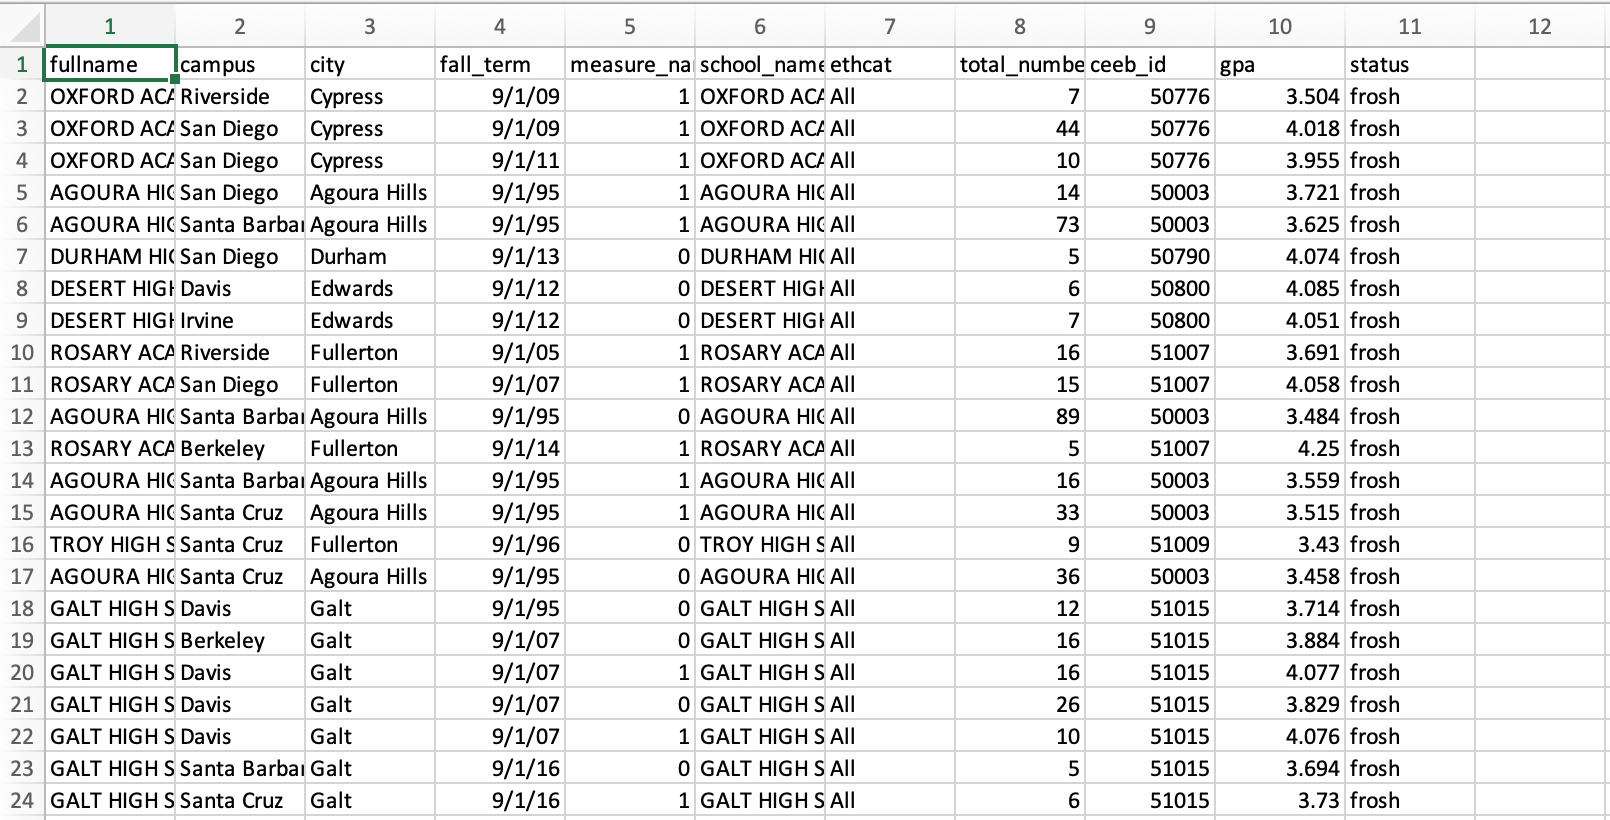
\includegraphics[width=100mm, scale=0.5]{images/ColumnHeader.png}
\end{center}

\section{Problem Description}
This problem can be easily simplified down to a two class classification problem with four parameters. An application can fall into one of two classes: admitted/accepted (1) or applied/rejected (0). The four parameters that affect their chances of falling into either class include: campus, year of enrollment, gpa, and status as a freshmen/transfer. To implement our logistic regression algorithm we used scikit learn, as well as pandas to manage and process the data we used. \newline
Our pandas workflow follows:
\begin{enumerate}
    \item Read our data in from the pre-processed csv file.
    \item Drop unwanted parameters.
    \item Create and concat dummy parameters for categorical variables.
\end{enumerate}
Our sklearn workflow follows:
\begin{enumerate}
    \item Split the data into testing and training sections and indicate the parameter to train for.
    \item [*2.] Create logistic regression object and indicate the solver, class weights, penalty, etc.
    \item Fit our data.
    \item Predict our testing data.
    \item Print the results.
\end{enumerate}

*: Despite trying every solver, weighting parameters, adjusting lambda, and penalization normalization we could not improve the performance of the model beyond that provided by the default values. \newline \newline 
\section{Methodology}
For the purpose of this project, we are not necessarily concerned about whether an admitted student actually enrolls in their chosen university, only if they will be admitted in the first place. By consolidating admissions decisions into whether an applicant was admitted or rejected, it becomes possible to make this prediction using classical logistic regression. \newline
%Cleaning the data
The first step to implementing a robust logistic regression model is to examine the data set that will be used to train it.
It is best if the input variables are independent of one another; that is, that there is very little correlation between the individual variables. This helps reduce unintended bias within the system, which  may not be accounted for otherwise. For example, it may be unwise to consider both high school GPA and SAT scores if we want academic performance to hold the same weight as other application characteristics, because they tend to be highly correlated \cite{Zarate}. Luckily, SAT scores were not present in the data set; this was in issue that we were cognizant of beforehand. On the other hand, a student's high school GPA and their year of admission are not highly correlated. Thus, they can both be used as inputs because they provide insight into separate components of the applicant's overall profile, as well as account for changing admissions standards. \newline
\begin{center}
  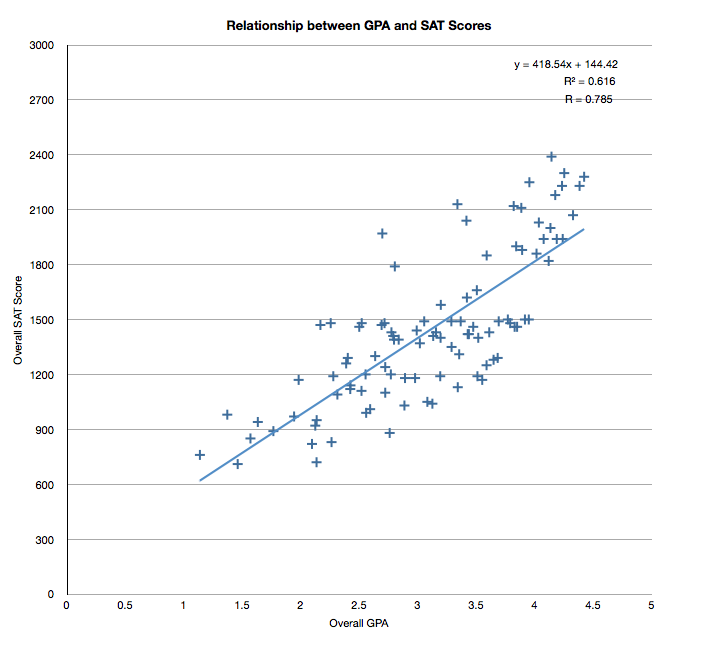
\includegraphics[width=100mm, scale=0.5]{images/SATvsGPA.png} \newline
  The figure above shows that high School GPA and SAT Scores are highly correlated, which gives this aspect of an applicant's performance more influence over their predicted chances of being admitted. This is not ideal for our model.
\end{center}
%Cleaning and Splitting the data
After ensuring that the input data is not interdependent and that the data is clean (e.g. eliminating entries where features are missing), we split all of the usable data into two parts. 80\% of the data was to be used to train the model, while the remaining 20\% of the data was to be used to test the accuracy of the trained model. To classify applicants into the "Admitted" or "Not Admitted" classes, we measure the output of the model's prediction against a classical sigmoid activation function.
\begin{center}
  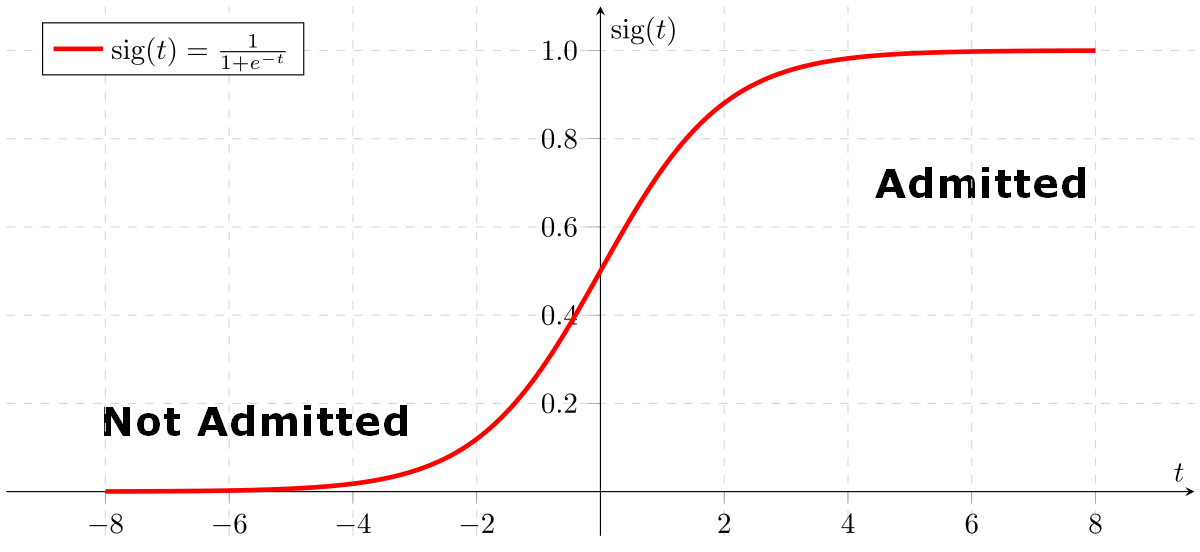
\includegraphics[width=100mm, scale=0.5]{images/Sigmoid.png} \newline
\end{center}
%Training
This model was trained on approximately 10 million entries. We initially fed a number of features into the model to predict each applicant's admissions status. These include the campus the applicant applied to, the intended year of enrollment, the GPA of the applicant, the applicant's status upon enrollment, and the student's ethnicity. It appears that the last input variable did not positively or negatively affect an applicant's chances of admission overall, so it was dropped from later training. \newline
\begin{center}
    \begin{tabular}{ |c|c|c|c| }
    \hline
    \multicolumn{4}{|c|}{450,000 ENTRIES} \\
    \hline
    \hline
    & PRECISION & RECALL & F1-SCORE \\
    \hline
    0 & 0.78 & 0.74 & 0.76 \\
    \hline
    1 & 0.77 & 0.81 & 0.79 \\
    \hline
    \hline
    ACCURACY & & & 0.78 \\
    \hline
    \end{tabular} \\
    Ethnicity and class status we found the results remained the same regardless.
\end{center}
%Estimating Loss
To gauge the accuracy of our trained classifier, we then compared the model's prediction to the ground truth supplied by the data set. We then altered various parameters of the logistic regression model such as the solver and regularization weight. This procedure was repeated many times to produce a well-trained model. \newline
%Testing
Once the training data could be modeled acceptably well, without succumbing to over-fitting, we ran the model on our remaining testing data to evaluate the ultimate efficacy of the model. If our model was able to correctly determine admissions status for 75\% of entries in the testing data, then we determined that our model was appropriately robust. \newline \newline 
\section{Results}
For our testing data set of 2.5 million entries, our logistic regression model achieved an accurate admissions decision of 81 percent. Below is a table showing the results of running data sets of various entry sizes through the trained model while we were still tuning it: \newline
\begin{center}
    \begin{tabular}{ |c|c|c|c| }
    \hline
    \multicolumn{4}{|c|}{1,000 ENTRIES} \\
    \hline
    \hline
    & PRECISION & RECALL & F1-SCORE \\
    \hline
    0 & 0.59 & 0.53 & 0.56 \\
    \hline
    1 & 0.72 & 0.77 & 0.74 \\
    \hline
    \hline
    ACCURACY & & & 0.68 \\
    \hline
    \end{tabular}
\end{center}

\begin{center}
    \begin{tabular}{ |c|c|c|c| }
    \hline
    \multicolumn{4}{|c|}{10,000 ENTRIES} \\
    \hline
    \hline
    & PRECISION & RECALL & F1-SCORE \\
    \hline
    0 & 0.67 & 0.35 & 0.46 \\
    \hline
    1 & 0.61 & 0.85 & 0.71 \\
    \hline
    \hline
    ACCURACY & & & 0.62 \\
    \hline
    \end{tabular}
\end{center}

\begin{center}
    \begin{tabular}{ |c|c|c|c| }
    \hline
    \multicolumn{4}{|c|}{500,000 ENTRIES} \\
    \hline
    \hline
    & PRECISION & RECALL & F1-SCORE \\
    \hline
    0 & 0.66 & 0.35 & 0.46 \\
    \hline
    1 & 0.59 & 0.84 & 0.69 \\
    \hline
    \hline
    ACCURACY & & & 0.61 \\
    \hline
    \end{tabular}
\end{center}
%Describe trends in the data
As shown above, there is an inverse relationship between the size of the testing pool and the model's overall accuracy. This does not indicate that our classifier was trained well. Fortunately, this inverse relationship disappeared once we trained the model on fewer parameters. We attribute this to the regularization performed during training. 
We also found that the parameter of the number of students with the same details was not being interpreted properly as the weight of each entry so we decided to edit our data set to account for this. Our final data set includes copies of each entry totaling the same as this parameter. This increased the size of our data set from 450,000 to 12,500,000 entries. \\
The final accuracies of our model are as follows:

\begin{center}
    \begin{tabular}{ |c|c|c|c| }
    \hline
    \multicolumn{4}{|c|}{12,500,000 ENTRIES} \\
    \hline
    \hline
    & PRECISION & RECALL & F1-SCORE \\
    \hline
    0 & 0.87 & 0.79 & 0.83 \\
    \hline
    1 & 0.72 & 0.83 & 0.77 \\
    \hline
    \hline
    ACCURACY & & & 0.81 \\
    \hline
    \end{tabular}
\end{center}
%Discuss consequences of the relationship described above
\section{Conclusions and Future Work}
The primary intent of this project was to explore a generalized approach for predicting admissions decisions for prospective undergraduates to the University of California system. On a large scale, the classification model discussed above can be used to project the size and composition of any university's incoming class.
%These next two lines could go in the introduction
The ability to reliably estimate these metrics have many possible implications for American universities.
For example, the amount of federal funding a university receives is partially tied to the student population; universities that serve a large percentage of minority students are eligible for more funding than those that do not. \newline \indent
It is also possible to extend this project to further suit the needs of public American universities. Instead of condensing the admissions data into a two-class problem based on admission status, future work may involve expanding the model to accommodate the three classes originally represented in the data set: applied, admitted, and enrolled. With this three-class paradigm, universities may be able to use past admissions data to predict whether a student will decide to enroll at that university once admitted. This is particularly important, again, for funding purposes. University scholarships and grants can only be offered to a small number of admitted students. While it is relatively easy to re-allocate funding that has been declined, it is much more difficult to deliver on funding that has been promised to too many students. A robust admissions-enrollment estimator would minimize the risk of over-promising funding while maximizing the efficiency of offering funding to students who are likely to enroll. \newline \indent
As with any technology that affects the lives of those who interact with it, there are certain challenges that come with assuring that the predictive model remains fair. It is important to note that this classification model is intended to supplement, rather than replace, the current admissions process. To fully automate the admissions process may be irresponsible, as undergraduate admissions rely on various qualitative application pieces that cannot be quantified without bias. This model can be useful for predicting admissions based on quantities like test scores, but should be used in conjunction with qualitative analyses of other application components like the personal statement and summary of past experiences. In addition, this model should be adjusted to fit the needs of the institution using it. Public American universities are marked with a distinct heterogeneity; the admissions needs of a small liberal arts college will differ greatly from those of a large research university. As such, it may be prudent to encourage thorough retraining of the model to fit past admissions data of the institution using it, to ensure that applicants are judged within reasonable standards.

\section{Theoretical Properties (Bonus)}
Property 1: We assume that all of the predictors are independent of one another, so we are basing our model on a classic Naive Bayes Classifier. Our algorithm relies on the idea that all of the predictors--from the applicant's GPA to their desired campus--are independent. In reality, we cannot guarantee that these predictors are independent; after all, people would not apply to a certain university if they know they did not have the minimum requisite qualifications. However, we make every effort to minimize the interdependence between predictors when we pre-process the data. In addition, we assume that our training data is not affected by extraneous factors, such as large-scale economic struggle and severe fluctuations in enrollment standards. \newline\newline\indent
Property 2: Theoretically, it is possible to derive the exact value that each input feature has for increasing an applicant's chance of admittance. These values are determined implicitly/retroactively by the admissions committees of the past and are computed by the classifier as it trains. If the exact values were discovered, an applicant would be able to concentrate on the most "valuable" component and artificially increase their chances of being admitted by the model's standards. \newline\newline\indent
Property 3: We assume that as the data updates, so does the training model. With an increase in entries the training model has a larger data set to use. This in turn allows for more accurate training, and eventually a more accurate model to test with. This can also be seen in our results section of the report, proving that the alterations of the algorithm led to this theoretical property.
\section{GitHub} \noindent
Below is a link to the open github repository. Here we have posted each of our proposals as we progressed, as well as the code for our final report. \newline\newline \indent
https://git.txstate.edu/h-r77/OCR-Project

\bibliographystyle{plain}
\bibliography{references}
\end{document}